\documentclass[11pt,letter, swedish, english,%twocolumn
]{article}
\pdfoutput=1

\usepackage[oldint]{../../custom_as}

\graphicspath{ {figures/} }

%\swapcommands{\Phi}{\varPhi}

%\renewcommand{\thesubsection}{\arabic{section} (\alph{subsection})}

%\renewcommand{\thesubsubsection}{\arabic{section} (\alph{subsection},\,\roman{subsubsection})}


%%Drar in tabell och figurtexter
\usepackage[margin=10 pt]{caption}
%%För att lägga in 'att göra'-noteringar i texten
\usepackage{todonotes} %\todo{...}

%%För att själv bestämma marginalerna. 
\usepackage[
            top    = 3cm,
%            bottom = 3cm,
            left   = 3cm, right  = 3cm
]{geometry}

\DeclareMathAlphabet{\mathpzc}{OT1}{pzc}{m}{it}
\newcommand{\oh}{\ensuremath\mathpzc{o}}

\newcommand{\as}{\qcomma\text{as }}

%\renewcommand{\thefootnote}{\fnsymbol{footnote}}




\usepackage{fancyhdr}
\pagestyle{fancy}
%\fancyhf{}
%\chead{\texttt{v.1.3}}
\lhead{Incomplete swing report}
\rhead{\today\quad\texttt{v.1.3}}
%\rfoot{Page \thepage}


\begin{document}

%%%%%%%%%%%%%%%%% vvv Inbyggd titelsida vvv %%%%%%%%%%%%%%%%%

% \title{\vspace{-2.5cm}Energy argument}
% \author{Andréas Sundström}
% \date{\today,\;\; \texttt{v\,1.4}}

%\maketitle

%%%%%%%%%%%%%%%%% ^^^ Inbyggd titelsida ^^^ %%%%%%%%%%%%%%%%%


\section{How to pump a swing}
A pendulums is one of the simplest physical systems -- we can all
understand, in broad terms, the behavior of pendulum set in
motion. However, a more intriguing scenario is when a child starts off
on a swing with virtually zero amplitude, and after just a few minutes
is swinging high and fast; and that without anyone pushing.
Consequently the main objective of this section is to explore how it
is possible to pump a swing \emph{without} any external forcing. 

One of the simplest models, put forth by Tea \& Falk in
1968~\cite{Tea_Falk_1968}, is the \emph{parametrically forced
  pendulum}, where the length of the pendulum varies to increase the
amplitude of the swing. The physical interpretation of this model is
that the child moves his center of mass (CM) up and down along the radial
direction of the swing. Also the child and the swing are viewed as a
point mass on a mass less connection to the swing suspension. 

In this section we will study the equation of motion for such a system,
then we study the energy of the swing in more detail to arrive at a
physical understanding of how the swing can gain energy through this
parametric forcing. We will study the cases where the length of the
pendulum is either directly dependent on time, or directly dependent
of the phase of the swing.
After that, we will use 
\todo{Specify later!}
perturbation techniques to study the motion of the swing.

\subsection{The equation of motion}
One of the most interesting parameters will be the angle, $\phi$,
the swing makes against the vertical as in \figref{fig:pendulum}. 
A simple and elegant way to find $\phi(t)$ is to use the Lagrangian
formalism. We therefore need to find the Lagrangian $\mathcal{L}=T-V$,
where $T$ is the kinetic energy and $V$ is the potential energy of the
swing. 

To find the kinetic energy, we will need to know the velocity of the
CM. Since we are looking for the angle, polar coordinates
are preferred. In polar coordinates the velocity is given by
$\vb{v}=\dot{l}\vu{r}+l\dot{\phi}\vu{\phi}$. Thus the kinetic energy is
\begin{equation}
T=\frac{m}{2}\vb{v}^2=\frac{m}{2}\qty(\dot{l}^2(t)+l^2(t)\dot{\phi}^2(t)).
\end{equation}
Next the potential energy can be written as
\begin{equation}
V=mg\,\Big[l_0-l(t)\cos\phi(t)\Big],
\end{equation}
where the zero point of the potential is set at the bottom of a
free-running swing -- i.e. a swing where $l(t)\equiv l_0$. 

\begin{figure}\centering
\resizebox{.2\textwidth}{!}{\input{figures/pendulum.pdf_t}}
\caption{A sketch of the pendulum and its movement (along the dotted
  curve) under influence of parametric forcing. the length of the
  pendulum is assumed to be of the 
form $l(t)=l_0[1+\epsilon\,\delta(t)]$, 
}
\label{fig:pendulum}
\end{figure}

By now using the Euler-Lagrange equation on $\mathcal{L}=T-V$, with
 respect to $\phi$ and $\dot\phi$, we get
\begin{equation}
0=\dv{t}\qty[\pdv{\mathcal{L}}{\dot{\phi}}]-\pdv{\mathcal{L}}{\phi}
=ml^2\ddot\phi +2ml\dot{l}\dot\phi +mgl\sin\phi.
\end{equation}
This can be cleaned up by dividing through by $m$ and $l$. 

To further simplify the equation of motion (EOM), we
non-dimensionalize by introducing
\begin{equation}\label{eq:non-dim}
l\to \frac{l}{l_0}=:r\qcomma\text{and}\quad
t\to\omega t.
%\tau=\omega t.
\end{equation}
Here $l_0$ is the average length of the pendulum, and $\omega$ is a
frequency that will be used in the forcing later -- i.e. $r(t)$ is a
periodic function with period $2\pi/\omega$. 
With the non-dimensionalized parameters we get the EOM:
\begin{equation}\label{eq:eom}
r\ddot\phi+2\dot{r}\dot\phi + \eta^2\sin\phi=0,
%r(\tau)\phi''(\tau)+2r'(\tau)\phi'(\tau) + \eta^2\sin\phi(\tau)=0,
\end{equation}
where %$(')=(\dv*{\tau})$, and
$\eta^2=\omega_0^2/\omega=(g/l_0)^2/\omega^2$ is the square of the
ratio of the free-running frequency $\omega_0$ to the forcing
frequency $\omega$. 



\subsection{The energy of the swing}
Non-dimenzionalizing $T$ and $V$ using \eqref{eq:non-dim}, % $r$ and $\tau$, 
and also dividing by $m$ because the mass has no significance here, we
get the non-dimensionalized energy  
\begin{equation}\label{eq:E}
E=\frac{1}{2}\qty[\dot{r}^2 + {r}^2\dot{\phi}^2] 
-\eta^2\Big[1-r\cos\phi\Big] 
\end{equation}
meaning that the time-derivative of the energy is
\begin{equation}
\begin{aligned}
\dv{E}{t}
=&\dot{r}\ddot{r}+r\dot\phi\qty(r\ddot\phi + \dot{r}\dot\phi + \eta^2\sin\phi) 
-\eta^2\dot{r}\cos\phi.
\end{aligned}
\end{equation}
No we note that the expression in parenthesis is just the LHS of
\eqref{eq:eom} with a term $r'\phi'$ missing. Therefore we can write
\begin{equation}\label{eq:dE/dt1}
\dv{E}{t}
=\dot{r}\ddot{r}+r\dot\phi\qty(0-\dot{r}\dot\phi)-\eta^2\dot{r}\cos\phi
=\dot{r}\ddot{r} - \dot{r}\qty(r\dot{\phi}^2 + \eta^2\cos\phi).
\end{equation}

% To get the pumped energy we integrate this over one
% period\footnotemark{}. But
% \begin{equation}
% \int_0^T\!\rd\tau r' r''=\qty[\frac{1}{2}{r'}^2]_0^T\approx0,
% \end{equation}
% meaning that we are left with:
% \begin{equation}\label{eq:int_dE1}
% \Delta{E}=-\int_0^T\!\rd\tau\;
% r'\qty(r{\phi'}^2 + \eta^2\cos\phi).
% \end{equation}

% \footnotetext{This is a little iffy, since we're not dealing with
%   perfectly periodic behavior, but hopefully it's manageable. }



\subsubsection{Physical interpretation of the swing energy}
\label{sec:phys_interp}
This has a really neat physical interpretation. When the child is
raising himself on the swing he has to do work against two forces:
the centrifugal and the gravitational force. Then since there's no
dissipation of energy, all the work done by the child must go into the
motion of the swing. 
The first term in the parenthesis in \eqref{eq:dE/dt1} corresponds
to the centrifugal force and the second term to the gravitational
force.
The term $\dot{r}\ddot{r}$ corresponds to the work needed to
accelerate the CM along the radius of the swing; this term will
however 
%\todo{This depends on how you want to define a ``cycle''.}approximately 
vanish over one cycle.\footnotemark{}  
\footnotetext{ 
Some amount of work is needed to accelerate the mass, but then the
same amount of energy is given back when the mass decelerates. 
Resulting in no net contribution to the swing energy over one cycle. }

By only looking at the reasoning above, without the need of the
analysis resulting in \eqref{eq:dE/dt1}, one can derive that in
order to pump the swing, the child must move inwards ($r'<0$) when the
swing is \emph{low}, and outwards ($r'>0$) when the swing is 
\emph{high}. The general shape of this movement is shown in
\figref{fig:pendulum}. 

% Because that would correspond to the child having to do the most
% amount of work against the two forces, and then letting the forces do
% the least amount of work. 

This is the reason why it's possible for the swing to gain energy by
only changing the length of the pendulum, and not having any external
forces. The child actually has to do work against the two forces when
moving the CM up, and then letting  the two forces do less work
when moving the CM down.

Furthermore, by actually studying the quantitative result,
\eqref{eq:dE/dt1}, we can conclude that the most effective pumping
is if $r$ abruptly decreases, the child stands \emph{up}, when
the swing is at its lowest ($\phi=0$), and then abruptly increases,
the child sits \emph{down}, when the swing is at its highest ($\phi$
is at its maximum). This strategy will result in an $r(t)$ that has a 
%\todo{Is is ok to use ``frequency'' (not sinusiodal)?}
frequency of about double that of the unperturbed swing --
i.e. $\omega\approx2\omega_0$ and $\eta\approx1/4$. 
This was also the case studied by Tea \& Falk~\cite{Tea_Falk_1968}.


% \subsubsection{Small angle approximation}
% If we limit ourselves to the small angle approximation, then
% $\cos(\phi)\approx1$ and 
% \begin{equation}
% \int_0^T\!\rd\tau\;r'\cos\phi
% \approx\int_0^T\!\rd\tau\;r'=0.
% \end{equation}
% The pumped energy now reduces to
% \begin{equation}
% \Delta{E}=-\int_0^T\!\rd\tau\;
% r'r{\phi'}^2.
% \end{equation}
% With $r=(1+\epsilon\,\delta{r})$ and $r'=\epsilon\,\delta{r'}$, we get
% \begin{equation}\label{eq:int_dE2}
% \Delta{E}=-\int_0^T\!\rd\tau\;r'{\phi'}^2
% +\order{\epsilon^2}.
% \end{equation}




\subsection{Studying some solutions}
\newcommand{\DE}{\Delta{E}}
There are two obvious ways to model the parametric forcing: either
having $r$ depend on time, or letting $r$ depend on the phase of the
swing. The strategy described above is an example of a phase dependent
forcing; that was also the most effective forcing. 
\todo{Update!}

% \vspace{11pt}
% \todo[inline]{%\noindent
% To do:\\
% %--- Find periodic solutions $\longrightarrow$ boundary between stable 
% %    and unstable regions.\\
% --- (Some plots of solutions)\\
% %--- Plot of Ince-Strutt diagram\\
% --- Insert more references.\\
% }


\subsubsection{Using energy considerations}
%\todo[inline]{This section has to be cut down! But I'ts very nice to
%  have this to start off of when going into the next section on doing
%  this with the \emph{method of multiple scales}.}
\todo{cut down!}
To get at feel for how the swing might behave we can begin by
calcuating the gained energy over one swing cycle:
\begin{equation}\label{eq:DE1}
\DE=\int_0^T\!\dv{E}{t}\id{t}
=-\int_0^T\! \dot{r}\qty(r\dot{\phi}^2 + \eta^2\cos\phi)\id{t}.
\end{equation}
Here we used \eqref{eq:dE/dt1} and the fact that the integral of
$\dot{r}\ddot{r}$ over one cycle is~$0$. 

Next we need to decide how to implement the forcing. From
section~\ref{sec:phys_interp} we learned that the most effective
forcing would occur when the forcing had double the frequency of the
free-running swing ($\eta=1/2$). As a first approximation we can use a purely time
dependent $r$, so a reasonalbe length would be
$ %\begin{equation}
r(t)=1+\epsilon\cos(t+t_0)
$ %\end{equation}
where $t_0$ is some constant phase shift, and $\epsilon\ll1$. 

Now, $\DE$ will be propotional to $\epsilon$, and thus $\DE\ll1$ as
well. This tells us that, to a first approximation, we can use the
unperturbed $\phi$ when calculating $\DE$. The unperturbed swing is
obtained by setting $\epsilon=0$ in the EOM, \eqref{eq:eom}, which
yields
\begin{equation}
\ddot\phi_0+\eta^2\,\sin\phi_0=0.
\end{equation}
We can choose the inital conditions to be $\phi_0(0)=a_0$ and
$\dot\phi_0(0)=0$. Next we restrict ourselves to $a_0\ll1$ so that we
can linearize the sine, which results in
\begin{equation}
\phi_0(t)=a_0\cos(\eta t)=a_0\cos(\frac{t}{2}).
\end{equation}

From here we substitute these results into \eqref{eq:DE1} and
integate. However, we can not integrate the last term, with a cosine
within a cosine; so we utilize the restriction $a_0\ll1$ to expand
$\cos(a_0\cos(t/2))\approx1-[a_0\cos(t/2)]^2/2$. We now end up with
\begin{equation}
\DE=+\epsilon\int_0^{4\pi}\!\!\sin(t+t_0)
\qty[\qty(-\frac{a_0}{2}\sin(t/2))^2
+\frac{1}{4}\qty(1-\frac{1}{2}\qty[a_0\cos(t/2)]^2)
]\id{t}+\order{\epsilon^2}.
\end{equation}
To simplify this we can rewrite the square of the sine and the cosine,
using the cosine double angle formula. Then use the fact that we are
integrating over two \emph{whole} periods of the sine in front,
meaning that any constats inside the brackets will
disappear. Eventually we get
\begin{equation}
\DE\approx
-\frac{3\epsilon a_0}{16}\int_0^{4\pi}\!\!\sin(t+t_0)\cos(t)\id{t}
=-\frac{3\pi\epsilon a_0}{8}\sin(t_0).
\end{equation}

From here it is clear that the most optimal forcing occurs with
$t_0=-\pi/2$, so that
\begin{equation}\label{eq:r}
r(t)=1+\epsilon\cos(t+t_0)=1+\epsilon\sin(t).
\end{equation}
This is also in good agreement with the reasoning in
section~\ref{sec:phys_interp}.

We can now study how the energy behaves over time. Using the
definition in \eqref{eq:E} we get $E_0=E(0)=a_0^2/8$ -- this can be
found by setting $t=\pi$ in \eqref{eq:E}. We can now write
\begin{equation}\label{eq:E(4pi)}
E(t=4\pi)=E(0)+\DE=(1+3\pi\epsilon)E_0.
\end{equation}
Since $\DE$ only depends on the energy at the start of the cycle it is
reasonable, when also regarding \eqref{eq:E(4pi)}, to assume an
exponential increas of $E$ in time. Using \eqref{eq:E(4pi)}, the
exponential behavoiur would then be
\begin{equation}
E(t)=E_0\exp[\ln(1+3\pi\epsilon)\frac{t}{4\pi}]
\approx E_0\,\ee^{\frac{3}{4}\epsilon t}.
\end{equation}
The angle of the swing, with the amplitude going as
$\sqrt{E}$, would therefore be 
\begin{equation}\label{eq:phi_from_E}
\phi(t)\approx a_0\ee^{\frac{3}{8}\epsilon t}\cos(t/2).
\end{equation}
At least for $t\le\order{\epsilon}$ -- after that non-linearities in the
original EOM would set in and disrupt the sync between $r(t)$ and
$\phi(t)$. 

% \subsubsection{Phase dependent forcing}
% From ones own experience or from observing how a child operates the
% playground swing, it's clear that the forcing is with response to the
% \emph{phase} of the swing. 
% One problem however with phase dependent
% forcing is that it will involve crucial non-linearities which makes a
% theoretical analysis very difficult.  


%\subsubsection{Time dependent forcing}

% One advantage of phase dependent forcing is that, then the forcing
% will always be in sync with the swing -- which is crucial to pump the
% swing. Since the swing is a non-linear pendulum the swing frequency
% will be amplitude dependent; this way a purely time dependent forcing,
% with fixed forcing frequency, can not stay in sync with a pumped swing
% and thus not pump it indefinitely. 
% However, for short time scales, time dependent forcing will still
% work. This is what we will study in this section.

% \vspace{11pt}
% \todo[inline]{\noindent
% Working with \eqref{eq:eom} doesn't seem to work, need to transform
% $\theta(\tau)=r(\tau)\phi(\tau)$ to get rid of first derivative.
% Then strain $\eta^2=\frac{1}{4}+\epsilon\eta_1^2+\epsilon^2\eta_2^2$
% to find boundary where solution is periodic. This relies on Floquet theory.\\
% \vspace{11pt}
% Probably won't have anything new in terms of perturbation techniques
% on the swing. What I've described above has already been done in the thesis.
% }

% \vspace{11pt}
% \todo[inline]{
% A completely new turn!\\
% I will here use the method of multiple scales to rederive
% \eqref{eq:phi_from_E}. 
% }

\subsubsection{Using the method of multiple scales}

In this section we will use the method of multiple scales to
rederive and improve the result from the previous section. In order to
use this method, we introduce a new timescale $\tau=\epsilon{t}$ and
the total derivatie becomes
\begin{equation}
\dv{t}=\pdv{t}+\epsilon\pdv{\tau}.
\end{equation}
With this the EOM becomes
\begin{equation}\label{eq:eom_mms}
\phi_{tt}+2\epsilon\phi_{t\tau}+\epsilon^2\phi_{\tau\tau}
+\frac{r_t}{r}(\phi_t+\epsilon\phi_\tau)+\frac{\eta^2}{r}\sin(\phi)=0,
\end{equation}
with the initial conditions 
\begin{equation}\label{eq:inti_mms}
\phi(0, 0)=a_0\ll1\qcomma
\phi_t(0, 0)+\epsilon\phi_\tau(0, 0)=0.
\end{equation} 
Note that only $r_t$ was used, since $r$ still only has $t$
dependence. 

Expanding \eqref{eq:eom_mms} up to $\order{\epsilon^2}$, using
\eqref{eq:r} and approximating $\sin(\phi)\approx\phi$, we get
\begin{equation}
\begin{aligned}
\phi_{tt}+2\epsilon\phi_{t\tau}+\epsilon^2\phi_{\tau\tau}+\eta^2\phi
=&\hspace{18pt}
\epsilon\qty[-2\cos(t)(\phi_t+\epsilon\phi_\tau)+\eta^2\sin(t)\phi]\\
&+\epsilon^2\qty[2\sin(t)\phi_t-2\eta^2\sin^2(t)\phi].
\end{aligned}
\end{equation}
Then we expand 
$\phi(t,\tau,\epsilon)=\phi_0(t,\tau)+
\epsilon\phi_1(t,\tau)+\epsilon^2\phi_0(t,\tau)+\ldots$ and use
$\eta=1/2$. This results in a series of DE's for each power of
$\epsilon$. 

The $\order{1}$ problem is just $\phi_{0,tt}+\phi_0/4=0$, which has the
solution
\begin{equation}
\phi_0(t,\tau)=A_0(\tau)\cos(t/2)+B_0(\tau)\sin(t/2).
\end{equation}
With the inital conditions $A_0(0)=a_0$ and $B_0(0)=0$.

Next the $\order{\epsilon}$ problem: 
\begin{equation}
\begin{aligned}
\phi_{1, tt}+\frac{1}{4}\phi_1=&\Big[A_{0,\tau}\sin(t/2)-B_{0, \tau}\cos(t/2)\Big]\\
&+\cos(t)\Big[A_0\sin(t/2)-B_0\cos(t/2)\Big]
+\frac{\sin(t)}{4}\Big[A_0\cos(t/2)+B_0\sin(t/2)\Big],
\end{aligned}
\end{equation}
which after reducing the multiplication of te trigonometric functions
reduces to
\begin{equation}
\begin{aligned}
\phi_{1, tt}+\frac{1}{4}\phi_1=&\phantom{+}A_{0,\tau}\sin(t/2)
-\frac{A_0}{8}\Big[3\sin(t/2)-5\sin(3t/2)\Big]\\
&{-}B_{0, \tau}\cos(t/2)
-\frac{B_0}{8}\Big[3\cos(t/2)+5\cos(3t/2)\Big].
\end{aligned}
\end{equation}
We see here that to remove the secular terms, we must have
\begin{equation}
\begin{cases}
A_0'-\frac{3}{8}A_0=0\qcomma&A_0(0)=a_0,\\
B_0'+\frac{3}{8}B_0=0\qcomma&B_0(0)=0,
\end{cases}
\end{equation}
which have the solutions $A_0(\tau)=a_0\ee^{\frac{3}{8}\tau}$ and
$B_0\equiv0$. And the solution to the $\order{\epsilon}$ problem
becomes
\begin{equation}
\phi_1(t, \tau)=A_1(\tau)\cos(t/2)+B_1(\tau)\sin(t/2)
-\frac{5}{16}A_0(\tau)\sin(3t/2).
\end{equation}
Using \eqref{eq:inti_mms}, the initial conditions are $A_1(0)=0$ and
$B_1(0)-15A_0(0)/32 + A_0'(0)=0$, which results in $B_1(0)=3a_0/32$.

Continuing on in an analogous way, the $\order{\epsilon^2}$ problem
will yield sekular temrs. The removal of which will result in a set of
DE's for $A_1$ and $B_1$. The details of these, quite laborious,
calculations are best suited for some kind of symbolic mathematical
program -- e.g. Mathematica. The DE's for $A_1$ and $B_1$ are 
\begin{equation}
\begin{cases}
128A_1'-48A_1=0\qcomma&A_1(0)=0\\
128B_1'+48B_1=-107a_0\ee^{\frac{3}{8}\tau}\qcomma&B_1(0)=\frac{3a_0}{32},
\end{cases}
\end{equation}
which have the solutions $A_1(\tau)\equiv0$ and
\begin{equation}
B_1(\tau)=\frac{a_0}{96}
\qty(116\ee^{-\frac{3}{8}\tau}-107\ee^{\frac{3}{8}\tau}).
\end{equation}

\paragraph{Results}
We now have a full solution up to $\order{\epsilon}$.
% \begin{equation}
% \phi(t)=a_0\ee^{\frac{3}{8}\tau}\cos(\frac{t}{2})
% +\frac{a_0\epsilon}{96}\qty[
% \qty(116\ee^{-\frac{3}{8}\tau}-107\ee^{\frac{3}{8}\tau})
% \sin(\frac{t}{2})
% -30\ee^{\frac{3}{8}\tau}\sin(\frac{3t}{2})]
% +\mathcal{O}_\text{F}\qty(\epsilon^2).
% \end{equation}
% \begin{equation}
% \begin{aligned}
% \phi(t, \tau)=&a_0\ee^{\frac{3}{8}\tau}\cos(t/2)\\
% &+\frac{a_0\epsilon}{96}\qty[
% \qty(116\ee^{-\frac{3}{8}\tau}-107\ee^{\frac{3}{8}\tau})
% \sin(t/2)
% -30\ee^{\frac{3}{8}\tau}\sin(3t/2)]
% +\mathcal{O}_\text{F}\qty(\epsilon^2).
% \end{aligned}
% \end{equation}
Going back to only $t$, we get
\begin{equation}
\phi(t)=a_0\ee^{\frac{3}{8}\epsilon{t}}\cos(\frac{t}{2})
+\frac{\epsilon a_0}{96}\ee^{\frac{3}{8}\epsilon{t}}\qty[
\qty(116\ee^{-\frac{3}{4}\epsilon{t}}-107)
\sin(\frac{t}{2})
-30\sin(\frac{3t}{2})]
{+}\mathcal{O}_\text{F}\qty(\epsilon^2)
% %\\=&
% a_0\ee^{\frac{3}{8}\epsilon{t}}\qty{
% \cos(\frac{t}{2})
% +\frac{\epsilon}{96}\qty[
% \qty(116\ee^{-\frac{3}{4}\epsilon{t}}-107)
% \sin(\frac{t}{2})
% -30\sin(\frac{3t}{2})]}
% +\mathcal{O}_\text{F}\qty(\epsilon^2)
% \end{aligned}
\end{equation}
We can now see that the first term is precisely what we had in
\eqref{eq:phi_from_E}. 



\subsubsection{Comparison to numerical simulations}

\todo[inline]{
There will be a plot here comparing \eqref{eq:phi_from_E} to numerical
simulations. And also discussing the break down of the previous
calculations. Maybe I'll even derive an expression for when the
approximations breaks down.
}

\begin{figure}\centering
%\resizebox{.2\textwidth}{!}{
% GNUPLOT: LaTeX picture with Postscript
\begingroup
  \makeatletter
  \providecommand\color[2][]{%
    \GenericError{(gnuplot) \space\space\space\@spaces}{%
      Package color not loaded in conjunction with
      terminal option `colourtext'%
    }{See the gnuplot documentation for explanation.%
    }{Either use 'blacktext' in gnuplot or load the package
      color.sty in LaTeX.}%
    \renewcommand\color[2][]{}%
  }%
  \providecommand\includegraphics[2][]{%
    \GenericError{(gnuplot) \space\space\space\@spaces}{%
      Package graphicx or graphics not loaded%
    }{See the gnuplot documentation for explanation.%
    }{The gnuplot epslatex terminal needs graphicx.sty or graphics.sty.}%
    \renewcommand\includegraphics[2][]{}%
  }%
  \providecommand\rotatebox[2]{#2}%
  \@ifundefined{ifGPcolor}{%
    \newif\ifGPcolor
    \GPcolortrue
  }{}%
  \@ifundefined{ifGPblacktext}{%
    \newif\ifGPblacktext
    \GPblacktexttrue
  }{}%
  % define a \g@addto@macro without @ in the name:
  \let\gplgaddtomacro\g@addto@macro
  % define empty templates for all commands taking text:
  \gdef\gplbacktext{}%
  \gdef\gplfronttext{}%
  \makeatother
  \ifGPblacktext
    % no textcolor at all
    \def\colorrgb#1{}%
    \def\colorgray#1{}%
  \else
    % gray or color?
    \ifGPcolor
      \def\colorrgb#1{\color[rgb]{#1}}%
      \def\colorgray#1{\color[gray]{#1}}%
      \expandafter\def\csname LTw\endcsname{\color{white}}%
      \expandafter\def\csname LTb\endcsname{\color{black}}%
      \expandafter\def\csname LTa\endcsname{\color{black}}%
      \expandafter\def\csname LT0\endcsname{\color[rgb]{1,0,0}}%
      \expandafter\def\csname LT1\endcsname{\color[rgb]{0,1,0}}%
      \expandafter\def\csname LT2\endcsname{\color[rgb]{0,0,1}}%
      \expandafter\def\csname LT3\endcsname{\color[rgb]{1,0,1}}%
      \expandafter\def\csname LT4\endcsname{\color[rgb]{0,1,1}}%
      \expandafter\def\csname LT5\endcsname{\color[rgb]{1,1,0}}%
      \expandafter\def\csname LT6\endcsname{\color[rgb]{0,0,0}}%
      \expandafter\def\csname LT7\endcsname{\color[rgb]{1,0.3,0}}%
      \expandafter\def\csname LT8\endcsname{\color[rgb]{0.5,0.5,0.5}}%
    \else
      % gray
      \def\colorrgb#1{\color{black}}%
      \def\colorgray#1{\color[gray]{#1}}%
      \expandafter\def\csname LTw\endcsname{\color{white}}%
      \expandafter\def\csname LTb\endcsname{\color{black}}%
      \expandafter\def\csname LTa\endcsname{\color{black}}%
      \expandafter\def\csname LT0\endcsname{\color{black}}%
      \expandafter\def\csname LT1\endcsname{\color{black}}%
      \expandafter\def\csname LT2\endcsname{\color{black}}%
      \expandafter\def\csname LT3\endcsname{\color{black}}%
      \expandafter\def\csname LT4\endcsname{\color{black}}%
      \expandafter\def\csname LT5\endcsname{\color{black}}%
      \expandafter\def\csname LT6\endcsname{\color{black}}%
      \expandafter\def\csname LT7\endcsname{\color{black}}%
      \expandafter\def\csname LT8\endcsname{\color{black}}%
    \fi
  \fi
  \setlength{\unitlength}{0.0500bp}%
  \begin{picture}(9636.00,4534.00)%
    \gplgaddtomacro\gplbacktext{%
      \csname LTb\endcsname%
      \put(744,768){\makebox(0,0)[r]{\strut{}$-1$}}%
      \put(744,2507){\makebox(0,0)[r]{\strut{}$0$}}%
      \put(744,4245){\makebox(0,0)[r]{\strut{}$1$}}%
      \put(888,528){\makebox(0,0){\strut{} 0}}%
      \put(1471,528){\makebox(0,0){\strut{} 100}}%
      \put(2054,528){\makebox(0,0){\strut{} 200}}%
      \put(2637,528){\makebox(0,0){\strut{} 300}}%
      \put(3219,528){\makebox(0,0){\strut{} 400}}%
      \put(3802,528){\makebox(0,0){\strut{} 500}}%
      \put(4385,528){\makebox(0,0){\strut{} 600}}%
      \put(192,2506){\rotatebox{-270}{\makebox(0,0){\strut{}Original EOM}}}%
      \put(2636,168){\makebox(0,0){\strut{}$t$}}%
    }%
    \gplgaddtomacro\gplfronttext{%
      \csname LTb\endcsname%
      \put(2530,3995){\makebox(0,0)[r]{\strut{}$\phi(t)$}}%
      \csname LTb\endcsname%
      \put(2530,3755){\makebox(0,0)[r]{\strut{}$\pm a_0\exp(3\epsilon{t}/8)$}}%
    }%
    \gplgaddtomacro\gplbacktext{%
      \csname LTb\endcsname%
      \put(5562,768){\makebox(0,0)[r]{\strut{}$-1$}}%
      \put(5562,2507){\makebox(0,0)[r]{\strut{}$0$}}%
      \put(5562,4245){\makebox(0,0)[r]{\strut{}$1$}}%
      \put(5706,528){\makebox(0,0){\strut{} 0}}%
      \put(6289,528){\makebox(0,0){\strut{} 100}}%
      \put(6872,528){\makebox(0,0){\strut{} 200}}%
      \put(7455,528){\makebox(0,0){\strut{} 300}}%
      \put(8037,528){\makebox(0,0){\strut{} 400}}%
      \put(8620,528){\makebox(0,0){\strut{} 500}}%
      \put(9203,528){\makebox(0,0){\strut{} 600}}%
      \put(5010,2506){\rotatebox{-270}{\makebox(0,0){\strut{}Linearized EOM}}}%
      \put(7454,168){\makebox(0,0){\strut{}$t$}}%
    }%
    \gplgaddtomacro\gplfronttext{%
      \csname LTb\endcsname%
      \put(7348,3995){\makebox(0,0)[r]{\strut{}$\phi_\text{lin}(t)$}}%
      \csname LTb\endcsname%
      \put(7348,3755){\makebox(0,0)[r]{\strut{}$\pm a_0\exp(3\epsilon{t}/8)$}}%
    }%
    \gplbacktext
    \put(0,0){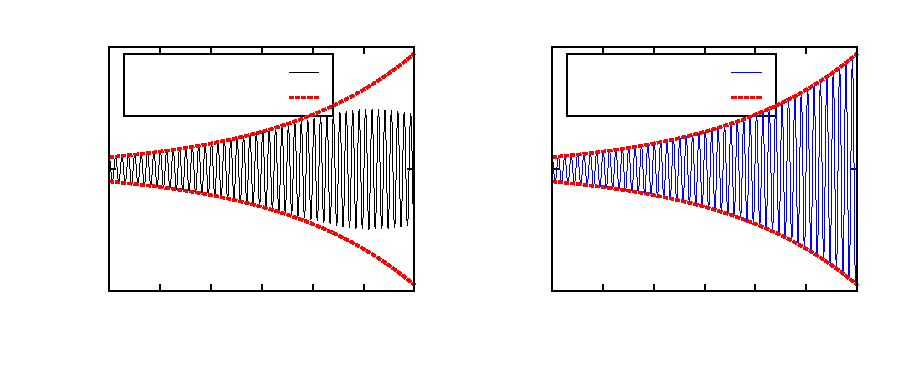
\includegraphics{swing_sim}}%
    \gplfronttext
  \end{picture}%
\endgroup
%}
\caption{Simulated swing angle, showing simulated results for both the
  original and the linearized EOM.
}
\label{fig:sim}
\end{figure}



\begin{thebibliography}{9}

\bibitem{Tea_Falk_1968}
Tea, P.L. Jr. and Falk, H. (1968). Pumping on a Swing. Am. J. Phys. 
\textit{36, 1165-6}

\bibitem{Strub_MSc_2009}
Strub, D.C. (2009). How do children swing?  M.Eng. thesis, University
of Bristol, Dept. of Eng. Math.%ematics

\end{thebibliography}


\end{document}




%  LocalWords:  parametrically EOM dimensionalize dimensionalized
%  LocalWords:  dimenzionalizing Floquet
